\documentclass[a4paper]{article}

\def\npart {IB}
\def\nterm {Lent}
\def\nyear {2016}
\def\nlecturer {I. Smith}
\def\ncourse {Complex Analysis}
\def\nlectures {MWF.11}
\def\nnotready {}

% Imports
\ifx \nextra \undefined
  \usepackage[pdftex,
    hidelinks,
    pdfauthor={Dexter Chua},
    pdfsubject={Cambridge Maths Notes: Part \npart\ - \ncourse},
    pdftitle={Part \npart\ - \ncourse},
  pdfkeywords={Cambridge Mathematics Maths Math \npart\ \nterm\ \nyear\ \ncourse}]{hyperref}
  \title{Part \npart\ - \ncourse}
\else
  \usepackage[pdftex,
    hidelinks,
    pdfauthor={Dexter Chua},
    pdfsubject={Cambridge Maths Notes: Part \npart\ - \ncourse\ (\nextra)},
    pdftitle={Part \npart\ - \ncourse\ (\nextra)},
  pdfkeywords={Cambridge Mathematics Maths Math \npart\ \nterm\ \nyear\ \ncourse\ \nextra}]{hyperref}

  \title{Part \npart\ - \ncourse \\ {\Large \nextra}}
\fi

\author{Lectured by \nlecturer \\\small Notes taken by Dexter Chua}
\date{\nterm\ \nyear}

\usepackage{alltt}
\usepackage{amsfonts}
\usepackage{amsmath}
\usepackage{amssymb}
\usepackage{amsthm}
\usepackage{booktabs}
\usepackage{caption}
\usepackage{enumitem}
\usepackage{fancyhdr}
\usepackage{graphicx}
\usepackage{mathtools}
\usepackage{microtype}
\usepackage{multirow}
\usepackage{pdflscape}
\usepackage{pgfplots}
\usepackage{siunitx}
\usepackage{tabularx}
\usepackage{tikz}
\usepackage{tkz-euclide}
\usepackage[normalem]{ulem}
\usepackage[all]{xy}

\pgfplotsset{compat=1.12}

\pagestyle{fancyplain}
\lhead{\emph{\nouppercase{\leftmark}}}
\ifx \nextra \undefined
  \rhead{
    \ifnum\thepage=1
    \else
      \npart\ \ncourse
    \fi}
\else
  \rhead{
    \ifnum\thepage=1
    \else
      \npart\ \ncourse\ (\nextra)
    \fi}
\fi
\usetikzlibrary{arrows}
\usetikzlibrary{decorations.markings}
\usetikzlibrary{decorations.pathmorphing}
\usetikzlibrary{positioning}
\usetikzlibrary{fadings}
\usetikzlibrary{intersections}
\usetikzlibrary{cd}

\newcommand*{\Cdot}{\raisebox{-0.25ex}{\scalebox{1.5}{$\cdot$}}}
\newcommand {\pd}[2][ ]{
  \ifx #1 { }
    \frac{\partial}{\partial #2}
  \else
    \frac{\partial^{#1}}{\partial #2^{#1}}
  \fi
}

% Theorems
\theoremstyle{definition}
\newtheorem*{aim}{Aim}
\newtheorem*{axiom}{Axiom}
\newtheorem*{claim}{Claim}
\newtheorem*{cor}{Corollary}
\newtheorem*{defi}{Definition}
\newtheorem*{eg}{Example}
\newtheorem*{fact}{Fact}
\newtheorem*{law}{Law}
\newtheorem*{lemma}{Lemma}
\newtheorem*{notation}{Notation}
\newtheorem*{prop}{Proposition}
\newtheorem*{thm}{Theorem}

\renewcommand{\labelitemi}{--}
\renewcommand{\labelitemii}{$\circ$}
\renewcommand{\labelenumi}{(\roman{*})}

\let\stdsection\section
\renewcommand\section{\newpage\stdsection}

% Strike through
\def\st{\bgroup \ULdepth=-.55ex \ULset}

% Maths symbols
\newcommand{\bra}{\langle}
\newcommand{\ket}{\rangle}

\newcommand{\N}{\mathbb{N}}
\newcommand{\Z}{\mathbb{Z}}
\newcommand{\Q}{\mathbb{Q}}
\renewcommand{\H}{\mathbb{H}}
\newcommand{\R}{\mathbb{R}}
\newcommand{\C}{\mathbb{C}}
\newcommand{\Prob}{\mathbb{P}}
\renewcommand{\P}{\mathbb{P}}
\newcommand{\E}{\mathbb{E}}
\newcommand{\F}{\mathbb{F}}
\newcommand{\cU}{\mathcal{U}}
\newcommand{\RP}{\mathbb{RP}}
\newcommand{\CP}{\mathbb{CP}}

\newcommand{\ph}{\,\cdot\,}

\DeclareMathOperator{\sech}{sech}
\DeclareMathOperator{\cosech}{cosech}
\DeclareMathOperator{\cosec}{cosec}

\DeclareMathOperator{\covol}{covol}
\DeclareMathOperator{\vol}{vol}

\let\Im\relax
\let\Re\relax
\DeclareMathOperator{\Im}{Im}
\DeclareMathOperator{\Re}{Re}
\DeclareMathOperator{\im}{im}
\DeclareMathOperator{\image}{image}
\DeclareMathOperator{\Ann}{Ann}

\DeclareMathOperator*{\res}{res}
\DeclareMathOperator{\Res}{Res}
\DeclareMathOperator{\Ind}{Ind}

\DeclareMathOperator{\tr}{tr}
\DeclareMathOperator{\diag}{diag}
\DeclareMathOperator{\rank}{rank}
\DeclareMathOperator{\card}{card}
\DeclareMathOperator{\spn}{span}
\DeclareMathOperator{\adj}{adj}

\DeclareMathOperator{\erf}{erf}
\DeclareMathOperator{\erfc}{erfc}

\DeclareMathOperator{\ord}{ord}
\DeclareMathOperator{\Sym}{Sym}

\DeclareMathOperator{\sgn}{sgn}
\DeclareMathOperator{\orb}{orb}
\DeclareMathOperator{\stab}{stab}
\DeclareMathOperator{\ccl}{ccl}

\DeclareMathOperator{\lcm}{lcm}
\DeclareMathOperator{\hcf}{hcf}

\DeclareMathOperator{\Int}{Int}
\DeclareMathOperator{\id}{id}

\DeclareMathOperator{\betaD}{beta}
\DeclareMathOperator{\gammaD}{gamma}
\DeclareMathOperator{\Poisson}{Poisson}
\DeclareMathOperator{\binomial}{binomial}
\DeclareMathOperator{\multinomial}{multinomial}
\DeclareMathOperator{\Bernoulli}{Bernoulli}
\DeclareMathOperator{\like}{like}

\DeclareMathOperator{\var}{var}
\DeclareMathOperator{\cov}{cov}
\DeclareMathOperator{\bias}{bias}
\DeclareMathOperator{\mse}{mse}
\DeclareMathOperator{\corr}{corr}

\DeclareMathOperator{\otp}{otp}
\DeclareMathOperator{\dom}{dom}

\DeclareMathOperator{\Root}{Root}
\DeclareMathOperator{\supp}{supp}
\DeclareMathOperator{\rel}{rel}
\DeclareMathOperator{\Hom}{Hom}
\DeclareMathOperator{\Aut}{Aut}
\DeclareMathOperator{\Gal}{Gal}
\DeclareMathOperator{\Mat}{Mat}
\DeclareMathOperator{\End}{End}
\DeclareMathOperator{\Char}{char}
\DeclareMathOperator{\ev}{ev}
\DeclareMathOperator{\St}{St}
\DeclareMathOperator{\Lk}{Lk}
\DeclareMathOperator{\disc}{disc}
\DeclareMathOperator{\Isom}{Isom}
\DeclareMathOperator{\length}{length}
\DeclareMathOperator{\energy}{energy}
\DeclareMathOperator{\area}{area}
\DeclareMathOperator{\Syl}{Syl}
\DeclareMathOperator{\cl}{cl}
\DeclareMathOperator{\fix}{fix}

\newcommand{\GL}{\mathrm{GL}}
\newcommand{\SL}{\mathrm{SL}}
\newcommand{\PGL}{\mathrm{PGL}}
\newcommand{\PSL}{\mathrm{PSL}}
\newcommand{\PSU}{\mathrm{PSU}}
\newcommand{\Or}{\mathrm{O}}
\newcommand{\SO}{\mathrm{SO}}
\newcommand{\U}{\mathrm{U}}
\newcommand{\SU}{\mathrm{SU}}

\renewcommand{\d}{\mathrm{d}}
\newcommand{\D}{\mathrm{D}}

\tikzset{->/.style = {decoration={markings,
                                  mark=at position 1 with {\arrow[scale=2]{latex'}}},
                      postaction={decorate}}}
\tikzset{<-/.style = {decoration={markings,
                                  mark=at position 0 with {\arrowreversed[scale=2]{latex'}}},
                      postaction={decorate}}}
\tikzset{<->/.style = {decoration={markings,
                                   mark=at position 0 with {\arrowreversed[scale=2]{latex'}},
                                   mark=at position 1 with {\arrow[scale=2]{latex'}}},
                       postaction={decorate}}}
\tikzset{->-/.style = {decoration={markings,
                                   mark=at position #1 with {\arrow[scale=2]{latex'}}},
                       postaction={decorate}}}
\tikzset{-<-/.style = {decoration={markings,
                                   mark=at position #1 with {\arrowreversed[scale=2]{latex'}}},
                       postaction={decorate}}}

\tikzset{circ/.style = {fill, circle, inner sep = 0, minimum size = 3}}
\tikzset{mstate/.style={circle, draw, blue, text=black, minimum width=0.7cm}}

\definecolor{mblue}{rgb}{0.2, 0.3, 0.8}
\definecolor{morange}{rgb}{1, 0.5, 0}
\definecolor{mgreen}{rgb}{0.1, 0.4, 0.2}
\definecolor{mred}{rgb}{0.5, 0, 0}

\def\drawcirculararc(#1,#2)(#3,#4)(#5,#6){%
    \pgfmathsetmacro\cA{(#1*#1+#2*#2-#3*#3-#4*#4)/2}%
    \pgfmathsetmacro\cB{(#1*#1+#2*#2-#5*#5-#6*#6)/2}%
    \pgfmathsetmacro\cy{(\cB*(#1-#3)-\cA*(#1-#5))/%
                        ((#2-#6)*(#1-#3)-(#2-#4)*(#1-#5))}%
    \pgfmathsetmacro\cx{(\cA-\cy*(#2-#4))/(#1-#3)}%
    \pgfmathsetmacro\cr{sqrt((#1-\cx)*(#1-\cx)+(#2-\cy)*(#2-\cy))}%
    \pgfmathsetmacro\cA{atan2(#2-\cy,#1-\cx)}%
    \pgfmathsetmacro\cB{atan2(#6-\cy,#5-\cx)}%
    \pgfmathparse{\cB<\cA}%
    \ifnum\pgfmathresult=1
        \pgfmathsetmacro\cB{\cB+360}%
    \fi
    \draw (#1,#2) arc (\cA:\cB:\cr);%
}
\newcommand\getCoord[3]{\newdimen{#1}\newdimen{#2}\pgfextractx{#1}{\pgfpointanchor{#3}{center}}\pgfextracty{#2}{\pgfpointanchor{#3}{center}}}

\def\Xint#1{\mathchoice
   {\XXint\displaystyle\textstyle{#1}}%
   {\XXint\textstyle\scriptstyle{#1}}%
   {\XXint\scriptstyle\scriptscriptstyle{#1}}%
   {\XXint\scriptscriptstyle\scriptscriptstyle{#1}}%
   \!\int}
\def\XXint#1#2#3{{\setbox0=\hbox{$#1{#2#3}{\int}$}
     \vcenter{\hbox{$#2#3$}}\kern-.5\wd0}}
\def\ddashint{\Xint=}
\def\dashint{\Xint-}


\begin{document}
\maketitle
{\small
\noindent\textbf{Analytic functions}\\
Complex differentiation and the Cauchy-Riemann equations. Examples. Conformal mappings. Informal discussion of branch points, examples of $\log z$ and $z^c$.\hspace*{\fill} [3]

\vspace{10pt}
\noindent\textbf{Contour integration and Cauchy's theorem}\\
Contour integration (for piecewise continuously differentiable curves). Statement and proof of Cauchy's theorem for star domains. Cauchy's integral formula, maximum modulus theorem, Liouville's theorem, fundamental theorem of algebra. Morera's theorem.\hspace*{\fill} [5]

\vspace{10pt}
\noindent\textbf{Expansions and singularities}\\
Uniform convergence of analytic functions; local uniform convergence. Differentiability of a power series. Taylor and Laurent expansions. Principle of isolated zeros. Residue at an isolated singularity. Classification of isolated singularities.\hspace*{\fill} [4]

\vspace{10pt}
\noindent\textbf{The residue theorem}\\
Winding numbers. Residue theorem. Jordan's lemma. Evaluation of definite integrals by contour integration. Rouch\'es theorem, principle of the argument. Open mapping theorem.\hspace*{\fill} [4]}

\tableofcontents
\section{Complex differentiation}
\subsection{Differentiation}
We first recall a few basic definitions. We are going to look at functions defined on subsets of the complex plane. Often, we just want to look at open subsets.
\begin{defi}[Open subset]
  A subset $U \subseteq \C$ is \emph{open} if for any $x \in U$, there is some $\varepsilon > 0$ such that the open ball $B_x(\varepsilon) = B(x; \varepsilon) \subseteq U$.
\end{defi}
The notation used for the open ball varies form time to time, even within the same sentence. For example, instead of putting $x$ as the subscript, we could put $\varepsilon$ as the subscript and $x$ inside the brackets. Hopefully, it will be clear from context.

\begin{defi}[Path-connected subset]
  A subset $U \subseteq \C$ is path-connected if for any $x, y \in U$, there is some $\gamma: [0, 1] \to U$ continuous such that $\gamma(0) = x$ and $\gamma(1) = y$.
\end{defi}

\begin{defi}[Domain]
  A \emph{domain} is a non-empty open path-connected subset of $\C$.
\end{defi}

Consider a domain $U \subseteq \C$ and a function $f: U \to \C$.
\begin{defi}[Differentiable function]
  We say a function $f$ is \emph{differentiable} at $w \in U$ if
  \[
    f'(w) = \lim_{z\to w} \frac{f(z) - f(w)}{z - w}
  \]
  exists.
\end{defi}
Here we implicitly require that the limit does not depend on which direction we approach $w$ from. It turns out this is a very strong condition to impose.

\begin{defi}[Analytic/holomorphic function]
  A function $f$ is \emph{analytic} or \emph{holomorphic} at $w \in U$ if $f$ is differentiable on an open neighbourhood $B(w, \varepsilon)$ of $w$.
\end{defi}

\begin{defi}[Entire function]
  If $f: \C \to \C$ is defined on all of $\C$ and is holomorphic on $\C$, then $f$ is said to be \emph{entire}.
\end{defi}

The goal of the course is to develop the rich theory of these complex differentiable functions and see how we can integrate them along continuously differentiable ($C^1$) paths in the complex plane.

First, we want to figure out when a function is differentiable. Given $f: U \to \C$, we can write it as $f = u + iv$, where $u, v: U \to \R$ are real-valued functions. Recall from IB Analysis II that a function $u: U \to \R$ viewed as a real-valued function of two variables is differentiable at a point $(c, d) \in U$, with derivative $Du|_{(c, d)} = (\lambda, \mu)$, if and only if
\[
  \frac{u(x, y) - u(c, d) - (\lambda (x - c) + \mu (y - d))}{\|(x, y) - (c, d)\|} \to 0
\]
as $(x, y) \to (c, d)$.

This allows us to come up with a nice criterion for when a function is differentiable
\begin{prop}
  Let $f$ be defined on an open set $U \subseteq \C$. Let $w = c + id \in U$ and write $f = u + iv$. Then $f$ is complex differentiable at $w$ if and only if $u$ and $v$ are differentiable at $(c, d)$, viewed as a real function of two real variables, \emph{and}
  \begin{align*}
    u_x &= v_y\\
    u_y &= -v_x
  \end{align*}
  These equations are the \emph{Cauchy-Riemann equations}. In this case, we have
  \[
    f'(w) = u_x(c, d) + iv_x(c, d) = v_y(c, d) -i u_y(c, d).
  \]
\end{prop}

\begin{proof}
  By definition, $f$ is differentiable at $w$ with $f'(w) = p + iq$ if and only if
  \[
    \lim_{z \to w} \frac{f(z) - f(w) - f'(w)(z - w)}{z - w} = 0. \tag{$\dagger$}
  \]
  If $z = x + iy$, then
  \[
    f'(w) (z - w) = p(x - c) - q(y - d) + i(q(x - c) + p (y - c)).
  \]
  So $(\dagger)$ holds if and only if
  \[
    \lim_{(x, y) \to (c, d)} \frac{u(x, y) - u(c, d) - (p(x - c) - q(y - d))}{\sqrt{(x - c)^2 + (y - d)^2}} = 0
  \]
  and
  \[
    \lim_{(x, y) \to (c, d)} \frac{v(x, y) - v(c, d) - (q(x - c) + p(y - d))}{\sqrt{(x - c)^2 + (y - d)^2}} = 0.
  \]
  Comparing this to the definition of the differentiability of a real-valued function, we see this holds exactly if $u$ and $v$ are differentiable at $(c, d)$ with
  \[
    Du|_{(c, d)} = (p, -q),\quad Dv|_{(c, d)} = (q, p).
  \]
\end{proof}
A standard warning is given that $f: U \to \C$ can be written as $f = u + iv$, where $u_x = v_y$ and $u_y = -v_x$ at $(c, d) \in U$, we \emph{cannot} conclude that $f$ is complex differentiable at $(c, d)$. These conditions only say the partial derivatives exist, but this does \emph{not} imply imply that $u$ and $v$ are differentiable, as required by the proposition. However, if the partial derivatives exist and are continuous, then by IB Analysis II we know they are differentiable.

\begin{eg}\leavevmode
  \begin{enumerate}
    \item A polynomial $p: \C \to \C$ is entire. This can be checked directly from definition.
    \item A \emph{rational function} $\frac{p(z)}{q(z)}: U \to \C$, where $U \subseteq \C \setminus \{z: q(z) = 0\}$, is holomorphic on any such $U$. Here $p, q$ are polynomials.
    \item $f(z) = |z|$ is \emph{not} complex differentiable at \emph{any} point of $\C$. Indeed, we can write this as $f = u + iv$, where
      \[
        u(x, y) = \sqrt{x^2 + y^2},\quad v(x, y) = 0.
      \]
      If $(x, y) \not= (0, 0)$, then
      \[
        u_x = \frac{x}{\sqrt{x^2 + y^2}},\quad u_y = \frac{y}{\sqrt{x^2 + y^2}}.
      \]
      If we are not at the origin, then clearly both cannot vanish, but the partials of $v$ both vanish. Hence the Cauchy-Riemann equations do not hold and it is not differentiable outside of the origin.

      At the origin, we can compute directly that
      \[
        \frac{f(h) - f(0)}{h} = \frac{|h|}{h}.
      \]
      This is, say, $+1$ for $h \in \R^+$ and $-1$ for $h \in \R^-$. So the limit as $h \to 0$ does not exists.
  \end{enumerate}
\end{eg}

\subsection{Conformal mappings}
The course schedules has a weird part where we are supposed to talk about conformal mappings for a lecture, but not use it anywhere else. We have to put them \emph{somewhere}, and we might as well do it now. However, this section will be slightly disconnected from the rest of the lectures.

\begin{defi}[Conformal function]
  Let $f: U \to \C$ be a function holomorphic at $w \in U$. If $f'(w) \not= 0$, we say $f$ is \emph{conformal}.
\end{defi}

Note that if $f = u + iv$, then viewed as a map $\R^2 \to \R^2$, we find the Jacobian matrix is
\[
  Df =
  \begin{pmatrix}
    u_x & u_y\\
    v_x & v_y
  \end{pmatrix}
\]
Then
\[
  \det (Df) = u_x v_y + u_y v_x = u_x^2 + u_y^2.
\]
Using the formula for the complex derivative in terms of the partials, this shows that if $f'(w) \not= 0$, then $\det(Df|_w) \not= 0$. Hence, by the inverse function theorem (viewing $f$ as a function $\R^2 \to \R^2$), $f$ is locally invertible at $w$.

It is an exercise to show that the usual rules of differentiation (sum, product, chain rule, derivative of inverse function) all hold for complex differentiation just as in the real case, with exactly the same proof. In particular, if a holomorphic function is conformal at a point $w$, then it has a local inverse which is also holomorphic and conformal.

Another useful property of conformal mappings is that they preserve angles. To give a precise statement of this, we need to specify how ``angles'' work.

The idea is to look at tangent vectors of paths. Let $\gamma_1, \gamma_2: [-1, 1] \to U$ be continuously differentiable paths that intersect when $t = 0$ at $w = \gamma_1(0) = \gamma_2(0)$. Moreover, assume $\gamma_i'(0) \not= 0$.

Then we can compare the angles between the paths by looking at the difference in arguments of the tangents at $w$. In particular, we define
\[
  \mathrm{angle} (\gamma_1, \gamma_2) = \arg (\gamma_1'(0)) - \arg (\gamma_2'(0)).
\]
(here we take $\arg$ to be the argument we would have if $w$ were the origin)

Let $f: U \to \C$ and $w \in U$. Suppose $f$ is conformal at $w$. Then $f$ maps our two paths to $f \circ \gamma_i: [-1, 1] \to \C$. These two paths now intersect at $f(w)$. Then the angle between them is
\begin{align*}
  \mathrm{angle} (f \circ \gamma_1, f\circ \gamma_2) &= \arg((f\circ \gamma_1)'(0)) - \arg((f \circ \gamma_2)'(0))\\
  &= \arg\left(\frac{(f\circ \gamma_1)'(0)}{(f \circ \gamma_2)'(0)}\right)\\
  &= \arg\left(\frac{\gamma_1'(0)}{\gamma_2'(0)}\right)\\
  &= \mathrm{angle} (\gamma_1, \gamma_2),
\end{align*}
using the chain rule and the fact that $f'(w) \not= 0$.

We will later prove that if $f: U \to \C$ is holomorphic on an open set $U$, then $f': U \to \C$ is \emph{also} holomorphic. Hence $f$ is infinitely differentiable.

Moreover, if we write $f = u + iv$, then using the formula for $f'$ in terms of the partials, we know $u$ and $v$ are also \emph{infinitely differentiable}. Differentiating the Cauchy-Riemann equations, we get
\[
  u_{xx} = v_{yx} = -u_{yy}.
\]
In other words,
\[
  u_{xx} + u_{yy} = 0,
\]
We get similar results for $v$ instead. Hence $\Re(f)$ and $\Im(f)$ satisfy the Laplace equation and are hence \emph{harmonic} (by definition).

\begin{defi}[Conformal equivalence]
  If $U$ and $V$ are open subsets of $\C$ and $f: U \to V$ is a conformal bijection, then it is a \emph{conformal equivalence}.
\end{defi}
Note that in general, a bijective continuous map need not have a continuous inverse. However, if we are given further that it is \emph{conformal}, then the inverse mapping theorem tells us there is a local conformal inverse, and if the function is bijective, these patch together to give a global conformal inverse.

\begin{eg}
  Any M\"obius map $A(z) = \frac{az + b}{cz + d}$ (with $ad - bc \not= 0$) defines a conformal equivalence $\C \cup \{\infty\} \to \C\cup \{\infty\}$ in the obvious sense. $A'(z) \not= 0$ follows from the chain rule and the invertibility of $A(z)$.

  In particular, the M\"obius group of the disk
  \begin{align*}
    \text{M\"ob}(D) &= \{f \in \text{M\"obius group}: f(D) = D\} \\
    &= \left\{\lambda\frac{z - a}{\bar{a}z - 1} \in \text{M\"ob} : |a| < 1, |\lambda| = 1\right\}
  \end{align*}
  is a group of conformal equivalences of the disk. You will prove that the M\"obius group of the disk is indeed of this form in the first example sheet.
\end{eg}
\begin{eg}
  The map $z \mapsto z^n$ for $n \geq 2$ is holomorphic everywhere and conformal except at $z = 0$. This gives a conformal equivalence
  \[
    \left\{z \in \C^*: 0 < \arg(z) < \frac{\pi}{n}\right\} \leftrightarrow \H,
  \]
  where we adopt the following notation:
\end{eg}

\begin{notation}
  We write $\C^* = \C \setminus \{0\}$ and
  \[
    \H = \{z \in \C: \Im (z) > 0\}
  \]
  is the upper half plane.
\end{notation}

\begin{eg}
  Note that $z \in \H$ if and only if $z$ is closer to $i$ than to $-i$. In other words,
  \[
    |z - i| < |z + i|,
  \]
  or
  \[
    \left|\frac{z - i}{z + i}\right| < 1.
  \]
  So $z \mapsto \frac{z - i}{z + i}$ defines a conformal equivalence $\H \to D$, the unit disc. We know this is conformal since it is a special case of the M\"obius map.
\end{eg}

\begin{eg}
  Consider the map
  \[
    z \mapsto w = \frac{1}{2}\left(z + \frac{1}{z}\right),
  \]
  assuming $z \in \C^*$. This can also be written as
  \[
    \frac{w + 1}{w - 1} = 1 + \frac{2}{w - 1} = 1 + \frac{4}{z + \frac{1}{z} - 2} = 1 + \frac{4z}{z^2 - 2z + 1} = \left(\frac{z + 1}{z - 1}\right)^2.
  \]
  So this is just squaring in some funny coordinates given by $\frac{z + 1}{z - 1}$. This map is holomorphic (except at $z = 0$). Also, we have
  \[
    f'(z) = 1 - \frac{z^2 + 1}{2z^2}.
  \]
  So $f$ is conformal except at $\pm 1$.

  Recall that the first thing we learnt about M\"obius maps is that they take lines and circles to lines and circles. This does something different. We write $z = re^{i\theta}$. Then if we write $z \mapsto w = u + iv$, we have
  \begin{align*}
    u &= \frac{1}{2}\left(r + \frac{1}{r}\right) \cos \theta\\
    v &= \frac{1}{2}\left(r - \frac{1}{r}\right) \sin \theta
  \end{align*}
  Fixing the radius and argument fixed respectively, we see that a circle of radius $\rho$ is mapped to the ellipse
  \[
    \frac{u^2}{\frac{1}{4}\left(\rho + \frac{1}{\rho}\right)^2} + \frac{v^2}{\frac{1}{4}\left(\rho - \frac{1}{\rho}\right)^2} = 1,
  \]
  while the half-line $\arg(z) = \mu$ is mapped to the hyperbola
  \[
    \frac{u^2}{\cos^2\mu} - \frac{v^2}{\sin^2 \mu} = 1.
  \]
  We can do something more interesting. Consider a off-centered circle, chosen to pass through the point $-1$ and $-i$. Then the image looks like this:
  \begin{center}
    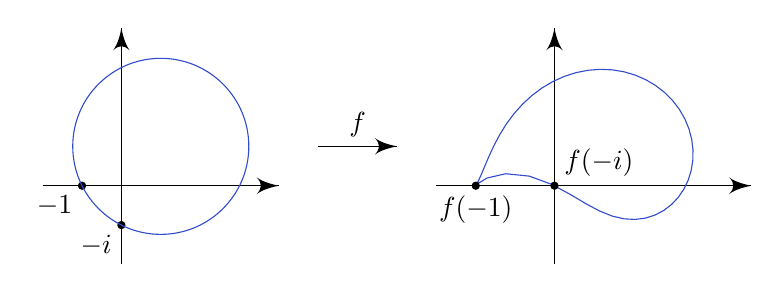
\begin{tikzpicture}[scale=0.5]
      \draw [->] (-2, 0) -- (4, 0);
      \draw [->] (0, -2) -- (0, 4);
      \node [circ] at (-1, 0) {};
      \node [circ] at (0, -1) {};
      \node at (-1, 0) [anchor = north east] {$-1$};
      \node at (0, -1) [anchor = north east] {$-i$};
      \draw [mblue] (1, 1) circle [radius=2.236];

      \draw [->] (5, 1) -- (7, 1) node [pos=0.5, above] {$f$};

      \begin{scope}[shift={(11, 0)}]
        \draw [->] (-3, 0) -- (5, 0);
        \draw [->] (0, -2) -- (0, 4);
        \draw [mblue, domain=0:360, samples=50] plot ({(sqrt (7 + 4.4721*(sin(\x) + cos(\x))) + 1/(sqrt (7 + 4.4721*(sin(\x) + cos(\x))))) * (2.236*cos(\x) + 1)/(sqrt (7 + 4.4721*(sin(\x) + cos(\x))))},{(sqrt (7 + 4.4721*(sin(\x) + cos(\x))) - 1/(sqrt (7 + 4.4721*(sin(\x) + cos(\x))))) * (2.236*sin(\x) + 1)/(sqrt (7 + 4.4721*(sin(\x) + cos(\x))))});
        \node [circ] at (-2, 0) {};
        \node [circ] at (0, 0) {};
        \node at (-2, 0) [below] {$f(-1)$};
        \node at (0, 0) [anchor = south west] {$f(-i)$};
      \end{scope}
    \end{tikzpicture}
  \end{center}
  Note that we have a singularity at $f(-1) = -1$. This is exactly the point where $f$ is not conformal, and is no longer required to preserve angles.

  This is a crude model of an aerofoil, and the transformation is known as the Joukowsky transform.

  In applied mathematics, this is used to model fluid flow over a wing in terms of the analytically simpler flow across a circular section. This is (apparently) useful because the Laplace's equation comes up a lot in fluid flow, and we have seen a connection between Laplace's equation and analytic functions.
\end{eg}

We interlude with a little trick. Often, there is no simple way to describe regions in space. However, if the region is bounded by circular arcs, there is a trick that can be useful.

Suppose we have a circular arc between $\alpha$ and $\beta$.
\begin{center}
  \begin{tikzpicture}
    \draw (0, 0) -- (8 ,0);
    \draw [dashed] (1, 0) -- (4, 2) -- (6, 0);
    \node [circ] (a) at (3, 1.333) {};
    \node [circ] (c) at (5, 1) {};
    \node [circ] (b) at (4, 2) {};
    \node at (a) [left] {$\alpha$};
    \node at (b) [above] {$z$};
    \node at (c) [right] {$\beta$};
    \drawcirculararc(5, 1)(4,2)(3, 1.333);

    \draw (1.4, 0) arc(0:33.69:0.4);
    \node [right] at (1.4, 0.2) {$\phi$};
    \draw (6.4, 0) arc(0:135:0.4);
    \node [right] at (6.4, 0.2) {$\theta$};
    \draw (4.2828, 1.7172) arc(315:213.69:0.4);
    \node [below] at (4, 1.6) {$\mu$};
  \end{tikzpicture}
\end{center}
Along this arc, $\mu = \theta - \phi = \arg(z - \alpha) - \arg(z - \beta)$ is constant. Thus, for each $\mu$, we get an arc from $\alpha$ to $\beta$.

To obtain a region bounded by two arcs, we find the two $\mu_-$ and $\mu_+$ that describe the boundary arcs. Then a point lie between the two arcs if and only if its $\mu$ is in between $\mu_-$ and $\mu_+$, ie. the region is
\[
  \left\{z: \arg\left(\frac{z - \alpha}{z - \beta}\right) \in [\mu_-, \mu_+]\right\}.
\]
This says the point has to lie in some arc between those given by $\mu_-$ and $\mu_+$.

For example, the following region:
\begin{center}
  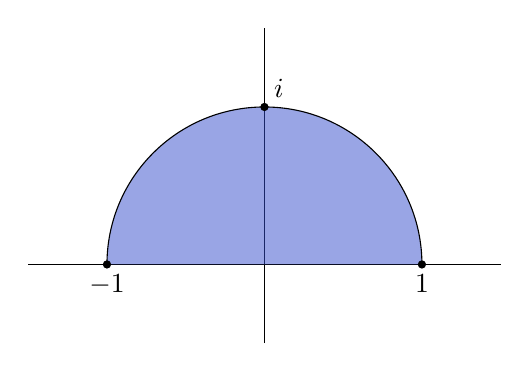
\begin{tikzpicture}
    \draw (-3, 0) -- (3, 0);
    \draw (0, -1) -- (0, 3);
    \fill [mblue, opacity=0.5] (2, 0) arc (0:180:2) -- (2, 0);
    \draw (2, 0) arc (0:180:2);
    \node [circ] at (-2, 0) {};
    \node [circ] at (2, 0) {};
    \node [circ] at (0, 2) {};
    \node at (-2, 0) [below] {$-1$};
    \node at (2, 0) [below] {$1$};
    \node at (0, 2) [anchor = south west] {$i$};
  \end{tikzpicture}
\end{center}
can be given by
\[
  \mathcal{U} = \left\{z: \arg\left(\frac{z - 1}{z + 1}\right) \in \left[\frac{\pi}{2}, \pi\right]\right\}.
\]
Thus for instance the map
\[
  z \mapsto -\left(\frac{z - 1}{z + 1}\right)^2
\]
is a conformal equivalence from $\mathcal{U}$ to $\H$. This is since if $z \in \mathcal{U}$, then $\frac{z - 1}{z + 1}$ has argument in $\left[\frac{\pi}{2}, \pi\right]$. Squaring doubles the angle and gives the lower half-plane, and multiplying by $-1$ gives the upper half plane.
\begin{center}
  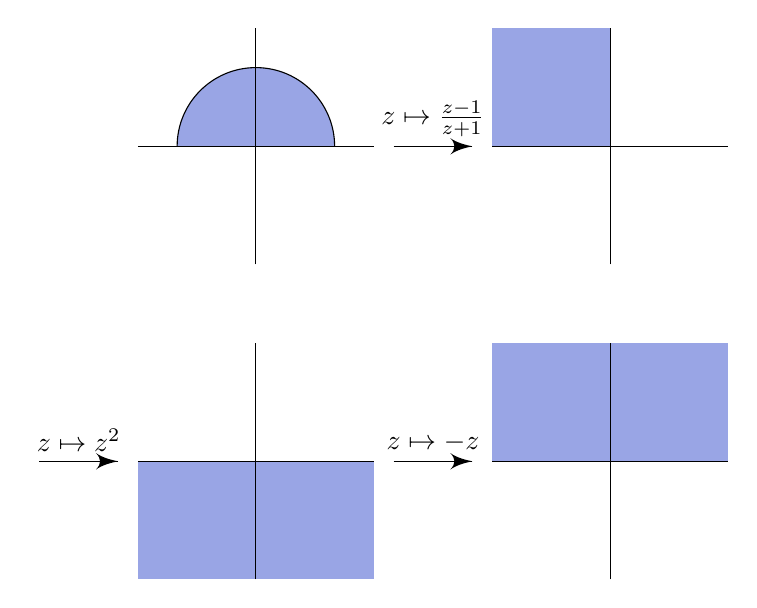
\begin{tikzpicture}[scale=0.5]
    \fill [mblue, opacity=0.5] (2, 0) arc (0:180:2) -- (2, 0);
    \draw (2, 0) arc (0:180:2);
    \draw (-3, 0) -- (3, 0);
    \draw (0, -3) -- (0, 3);

    \draw [->] (3.5, 0) -- (5.5, 0) node [pos=0.5, above] {$z \mapsto \frac{z - 1}{z + 1}$};
    \begin{scope}[shift={(9,0)}]
      \fill [mblue, opacity=0.5] (-3, 3) rectangle (0, 0);
      \draw (-3, 0) -- (3, 0);
      \draw (0, -3) -- (0, 3);

    \end{scope}
    \begin{scope}[shift={(0,-8)}]
      \draw [->] (-5.5, 0) -- (-3.5, 0) node [pos=0.5, above] {$z \mapsto z^2$};

      \fill [mblue, opacity=0.5] (-3, 0) rectangle (3, -3);
      \draw (-3, 0) -- (3, 0);
      \draw (0, -3) -- (0, 3);

      \draw [->] (3.5, 0) -- (5.5, 0) node [pos=0.5, above] {$z \mapsto -z$};
    \end{scope}
    \begin{scope}[shift={(9,-8)}]
      \fill [mblue, opacity=0.5] (-3, 0) rectangle (3, 3);
      \draw (-3, 0) -- (3, 0);
      \draw (0, -3) -- (0, 3);
    \end{scope}
  \end{tikzpicture}
\end{center}
In fact, there is a really powerful theorem telling us most things are conformally equivalent to the unit disk.

\begin{thm}[Riemann mapping theorem]
  Let $\mathcal{U} \subseteq \C$ be the bounded domain enclosed by a simple closed curve, or more generally any simply connected domain not equal to all of $\C$. Then $\mathcal{U}$ is conformally equivalent to $D = \{z: |z| < 1\} \subseteq \C\}$.
\end{thm}
This in particular tells us any two simply connected domains are conformally equivalent.

\begin{defi}[Simple closed curve]
  A \emph{simple closed curve} is the image of an injective map $S^1 \to \C$.
\end{defi}
It should be clear (though not trivial to prove) that a simple closed curve separates $\C$ into a bounded part and an unbounded part.

The more general statement requires the following definition:
\begin{defi}[Simply connected]
  A domain $\mathcal{U}\subseteq \C$ is \emph{simply connected} if every continuous map from the circle $f: S^1 \to \mathcal{U}$ can be extended to a continuous map from the disk $F: \overline{D^2} \to \mathcal{U}$ such that$F|_{\partial \overline{D^2}} = f$. Alternatively, any loop can be continuously shrunk to a point.
\end{defi}

\begin{eg}
  The unit disk is simply-connected, but the region defined by $1 < |z| < 2$ is not, since the circle $|z| = 1.5$ cannot be extended to a map from a disk.
  \begin{center}
    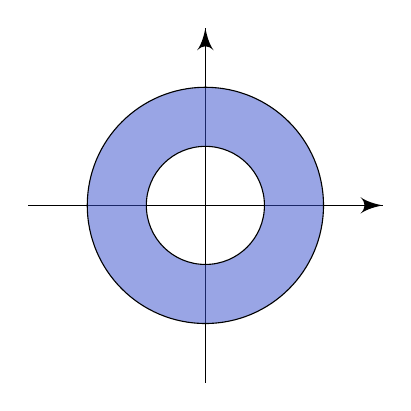
\begin{tikzpicture}[scale=0.75]
      \draw [->] (-3, 0) -- (3, 0);
      \draw [->] (0, -3) -- (0, 3);
      \fill [mblue, opacity=0.5] circle [radius=2];
      \fill [white] circle [radius=1];
      \draw circle [radius=1];
      \draw circle [radius=2];
      \draw (-1, 0) -- (1, 0);
      \draw (0, -1) -- (0, 1);
    \end{tikzpicture}
  \end{center}
\end{eg}
We will not prove this statement, but it is nice to know that this is true.

If we believe that the unit disk is relatively simple, then since all simply connected regions are conformally equivalent to the disk, all simply connected domains are boring. This suggests we will later encounter domains with holes to make the course interesting. This is in fact true, and we will study these holes in depth later.

\begin{eg}
  The exponential function
  \[
    e^z = 1 + z + \frac{z^2}{2!} + \frac{z^3}{3!} + \cdots
  \]
  defines a function $\C \to \C^*$. In fact it is a conformal mapping. This sends the region $\{z: \Re(z) \in [a, b]\}$ to the annulus $\{e^a \leq |w| \leq e^b\}$. One is simply connected, but the other is not --- this is not a problem since $e^z$ is \emph{not} bijective on the strip.
  \begin{center}
    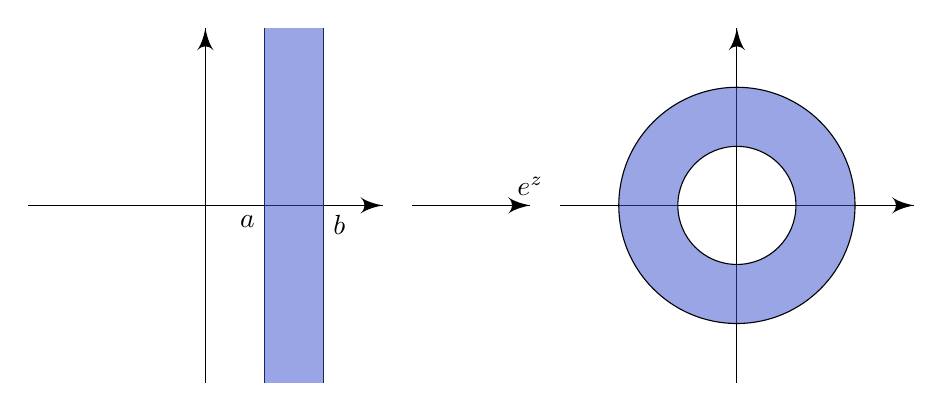
\begin{tikzpicture}[scale=0.75]
      \draw [->] (-3, 0) -- (3, 0);
      \draw [->] (0, -3) -- (0, 3);

      \draw (1, 3) -- (1, -3);
      \draw (2, 3) -- (2, -3);
      \fill [mblue, opacity=0.5] (1, 3) rectangle (2, -3);
      \node [anchor=north east] at (1, 0) {$a$};
      \node [anchor=north west] at (2, 0) {$b$};

      \draw [->] (3.5, 0) -- (5.5, 0) node [above] {$e^z$};
      \begin{scope}[shift={(9, 0)}]
        \draw [->] (-3, 0) -- (3, 0);
        \draw [->] (0, -3) -- (0, 3);
        \fill [mblue, opacity=0.5] circle [radius=2];
        \fill [white] circle [radius=1];
        \draw circle [radius=1];
        \draw circle [radius=2];
        \draw (-1, 0) -- (1, 0);
        \draw (0, -1) -- (0, 1);
      \end{scope}
    \end{tikzpicture}
  \end{center}
\end{eg}

\subsection{Power series and logarithms}
At this point, we need to recall some facts from IB Analysis II.
\begin{defi}[Uniform convergence]
  A sequence $(f_n)$ of functions \emph{converge uniformly} to $f$ if for all $\varepsilon > 0$, there is some $N$ such that $n > N$ implies $|f_n(z) - f(z)| < \varepsilon$ for all $z$.
\end{defi}

\begin{prop}
  The uniform limit of continuous functions is continuous.
\end{prop}

We also had the following nice test for uniform convergence of a series:
\begin{prop}[Weierstrass M-test]
  For a sequence of functions $f_n$, if we can find $(M_n) \subseteq \R_{>0}$ such that $|f_n(x)| < M_n$ for all $x$ in the domain, then $\sum M_n$ converges implies $\sum f_n(x)$ converges uniformly on the domain.
\end{prop}

Finally, we have the following result.
\begin{prop}
  Given any constants $\{c_n\}_{n \geq 0} \subseteq \C$, there is a unique $R \in [0, \infty]$ such that the series $z \mapsto \sum_{n = 0}^\infty c_n(z - a)^n$ converges absolutely if $|z - a| < R$ and diverges if $|z - a| > R$. Moreover, if $0 < r < R$, then the series converges uniformly on $|z| < r$. This $R$ is known as the \emph{radius of convergence}.
\end{prop}
So while we don't necessarily get uniform convergence on the whole domain, we get uniform convergence on all compact subsets of the domain.

We are now going to look at power series. They will serve as examples, and as we will see later, universal examples, of holomorphic functions.

\begin{thm}
  Let
  \[
    f(z) = \sum_{n = 0}^\infty c_n (z - a)^n
  \]
  be a power series with radius of convergence $R > 0$. Then
  \begin{enumerate}
    \item $f$ is holomorphic on $B(a; R) = \{z: |z - a| < R\}$.
    \item $f'(z) = \sum n c_n (z - 1)^{n - 1}$, which also has radius of convergence $R$.
    \item Therefore $f$ is infinitely complex differentiable on $B(a; R)$. Furthermore,
      \[
        c_n = \frac{f^{(n)}(a)}{n!}.
      \]
  \end{enumerate}
\end{thm}

\begin{proof}
  Without loss of generality, take $a = 0$. The third part obviously follows from the previous two, and we will prove the first two parts simultaneously. We would like to first prove that the series has radius of convergence $R$, so that we can freely happily manipulate it.

  Certainly, we have $|n c_n| \geq |c_n|$. So by comparison to the series for $f$, we can see that the radius of convergence of $\sum n c_n z^{n - 1}$ is at most $R$. But if $|z| < \rho < R$, then we can see
  \[
    \frac{|n c_n z^{n - 1}|}{|c_n \rho^{n - 1}|} = n \left|\frac{z}{\rho}\right|^{n - 1} \to 0
  \]
  as $n \to \infty$. So by comparison to $\sum c_n \rho^{n - 1}$, which converges, we see that the radius of convergence of $\sum n c_n z^{n - 1}$ is at least $\rho$. So the radius of convergence must be exactly $R$.

  Now we want to show $f$ really is differentiable with that derivative. Pick $z, w$ such that $|z|, |w| \leq \rho$ for some $\rho < R$ as before.

  Define a new function
  \[
    \varphi (z, w) = \sum_{n = 1}^\infty c_n \sum_{j = 0}^{n - 1} z^j w^{n - 1 - j}.
  \]
  Noting
  \[
    \left|c_n \sum_{j = 0}^{n - 1} z^j w^{n - 1 - j}\right| \leq n |c_n| \rho^n,
  \]
  we know the series defining $\varphi$ converges uniformly on $\{|z| \leq \rho, |w| < \rho\}$, and hence to a continuous limit.

  If $z \not= w$, then using the formula for the (finite) geometric series, we know
  \[
    \varphi(z, w) = \sum_{n = 1}^\infty c_n\left(\frac{z^n - w^n}{z - w}\right) = \frac{f(z) - f(w)}{z - w}.
  \]
  On the other hand, if $z = w$, then
  \[
    \varphi(z, z) = \sum_{n = 1}^\infty c_n n z^{n - 1}.
  \]
  Since $\varphi$ is continuous, we know
  \[
    \lim_{w \to z} \frac{f(z) - f(w)}{z - w} \to \sum_{n = 1}^\infty c_n nz^{n - 1}.
  \]
  So $f'(z) = \varphi(z, z)$ as claimed. Then (iii) follows from (i) and (ii) directly.
\end{proof}

\begin{cor}
  Given a power series
  \[
    f(z) = \sum_{n \geq 0} c_n (z - a)^n
  \]
  with radius of convergence $R > 0$, and given $0 < \varepsilon < R$, if $f$ vanishes on $B(a, \varepsilon)$, then $f$ vanishes identically.
\end{cor}

\begin{proof}
  If $f$ vanishes on $B(a, \varepsilon)$, then all its derivatives vanish, and hence the coefficients all vanish. So it is identically zero.
\end{proof}
This is obviously true, but will come up useful some time later.

It is might be useful to have an explicit expression for $R$. For example, we can have
\begin{align*}
  R &= \sup \{r \geq 0: |c_n|r^n \to 0\text{ as }n \to \infty\}\\
  &= \frac{1}{\limsup \sqrt[n]{|c_n|}}.
\end{align*}
But we probably won't need these.

Recall that the exponential function
\[
  e^z = \exp(z) = 1 + z + \frac{z^2}{2!} + \frac{z^3}{3!} + \cdots
\]
has a radius of convergence of $\infty$. So it is an entire function. We have the usual standard properties, such as $e^{z + w} = e^z e^w$, and also
\[
  e^{x + iy} = e^x e^{iy} = e^x(\cos y + i \sin y).
\]
So given $w \in \C^* = \C\setminus\{0\}$, there are solutions to $e^z = w$. In fact, this has infinitely many solutions, differing by adding integer multiples of $2\pi i$. In particular, $e^z = 1$ if and only if $z$ is an integer multiple of $2\pi i$.

This means we have to be a bit more careful if we want to talk about the inverse function of the exponential. We make the following definition:

\begin{defi}[Branch of logarithm]
  Let $U \subseteq \C^*$ be an open subset. A \emph{branch of the logarithm} on $U$ is a continuous function $\lambda: U \to \C$ for which $e^{\lambda (z)} = z$ for all $z \in U$.
\end{defi}
This is like a ``local inverse'' to the exponential function. These need not exist for all $U$. For example, there is no branch of the logarithm on the whole $\C^*$, as we will later prove.

\begin{eg}
  Let $U = \C\setminus \R_{\leq 0}$, a ``slit plane''.
  \begin{center}
    \begin{tikzpicture}
      \draw [->] (0, 0) -- (2, 0);
      \draw [thick] (-2, 0) -- (0, 0);
      \draw [->] (0, -2) -- (0, 2);
      \node [circ] at (0, 0) {};
    \end{tikzpicture}
  \end{center}
  Then for each $z \in U$, we write $z = r^{i \theta}$, with $-\pi < \theta < \pi$. Then $\lambda(z) = \log (r) + i \theta$ is a branch of the logarithm. This is the \emph{principal branch}.

  On $U$, there is a continuous function $\arg: U \to (-\pi, \pi)$, which is why we can construct a branch. This is not true on, say, the unit circle.
\end{eg}

\begin{prop}
  On $\{z \in \C: z \not\in \R_{\leq 0}\}$, the principal branch $\log: U \to \C$ is holomorphic function. Moreover,
  \[
    \frac{\d}{\d z}\log z = \frac{1}{z}.
  \]
  If $|z| < 1$, then
  \[
    \log (1 + z) = \sum_{n \geq 1} (-1)^{n - 1} \frac{z^n}{n} = z - \frac{z^2}{2} + \frac{z^3}{3} - \cdots.
  \]
\end{prop}

\begin{proof}
  That logarithm is holomorphic follows from the chain rule and $e^{\log z} = z$. This shows $\frac{\d}{\d z} (\log z) = \frac{1}{z}$.

  To show that $\log(1 + z)$ is indeed given by the said power series, note that the power series does have a radius of convergence $1$ by, say, the ratio test. So by the previous result, it has derivative
  \[
    1 - z + z^2 + \cdots = \frac{1}{1 + z}.
  \]
  Therefore, $\log(1 + z)$ and the power series have equal derivative, and hence coincide up to a constant. Since they agree at $z = 0$, they must in fact be equal.
\end{proof}
Note that if $\alpha \in \C$ and $\log: U \to \C$ is a branch of the logarithm, we can define
\[
  z^{\alpha} = e^{\alpha \log z}
\]
on $U$.

We can view $\log$ as a multivalued function on $\C^*$. In general, we say that a point $p \in \C $ is a \emph{branch point} of a multivalued function if the function cannot be given a continuous single-valued definition in a (punctured) neighbourhood $B(p, \varepsilon) \setminus \{p\}$ of $p$ for any $\varepsilon > 0$. For example, $0$ is a branch point of $\log$.

\begin{eg}
  Consider the function
  \[
    f(z) = \sqrt{z(z - 1)}.
  \]
  This has \emph{two} branch points, $z = 0$ and $z = 1$, since we cannot consistently a square root consistently near $0$, as it is defined via the logarithm.
\end{eg}

Note we can define a continuous branch of $f$ on either
\begin{center}
  \begin{tikzpicture}
    \draw [->] (-2, 0) -- (2, 0);
    \draw [thick] (-2, 0) -- (0, 0);
    \draw [thick] (1, 0) -- (2, 0);
    \draw [->] (0, -2) -- (0, 2);
    \node [below] at (1, 0) {$1$};
    \node [anchor = north east] {$0$};
    \node [circ] at (1, 0) {};
    \node [circ] at (0, 0) {};
  \end{tikzpicture}
\end{center}
or we can just kill a finite slit by
\begin{center}
  \begin{tikzpicture}
    \draw [->] (-2, 0) -- (2, 0);
    \draw [thick] (1, 0) -- (0, 0);
    \draw [->] (0, -2) -- (0, 2);
    \node [below] at (1, 0) {$1$};
    \node [anchor = north east] {$0$};
    \node [circ] at (1, 0) {};
    \node [circ] at (0, 0) {};
  \end{tikzpicture}
\end{center}
Why is the second case possible? Note that
\[
  f(z) = e^{\frac{1}{2}(\log(z) + \log(z - 1))}.
\]
If we move around a path encircling the finite slit, the argument of each of $f(z)$ and $\log(z - 1)$ will jump by $2\pi i$, and the total change in the exponent is $2\pi i$. So the expression for $f(z)$ becomes uniquely defined.

While these two ways of cutting slits look rather different, if we consider this to be on the Riemann sphere, then these two cuts now look similar. It's just that one passes through the point $\infty$, and the other doesn't.

However, this is not a very good treatment of the problem. A better treatment will be performed in the IID Riemann Surfaces course.

\section{Contour integration}
Our next task is to develop a theory of integration of $\C$-valued functions along paths and closed contours. At first, this would look just like an obvious generalization of real integration. However, this will suddenly become amazing and get a life of its own when we get to Cauchy's theorem.

Recall that a function $f: [a, b] \to \C$ is Riemann integrable if $\Re(f)$ and $\Im (f)$ are individually, by definition. Also, by definition,
\[
  \int_a^b f(t) \;\d t = \int_a^b \Re(f(t))\;\d t + i \int_a^b \Im(f(t))\;\d t.
\]
Recall also that if $f$ is continuous, then it is integrable. This will apply in most cases we care about in this course. After all, this is not a course on exotic functions.

We start from some less interesting facts, and slowly develop and prove some really amazing results.
\begin{lemma}
  Suppose $f: [a, b] \to \C$ is continuous (and hence integrable). Then
  \[
    \left|\int_a^b f(t)\;\d t\right| \leq (b - a) \sup_t |f(t)|
  \]
  with equality if and only if $f$ is constant.
\end{lemma}

\begin{proof}
  We let
  \[
    \theta = \arg\left(\int_a^b f(t)\;\d t\right),
  \]
  and
  \[
    M = \sup_t |f(T)|.
  \]
  Then we have
  \begin{align*}
    \left|\int_a^b f(t)\;\d t\right| &= \int_a^b e^{-i\theta} f(t)\;\d t\\
    &= \int_a^b \Re(e^{-i\theta} f(t))\;\d t\\
    &\leq (b - a) M,
  \end{align*}
  with equality if and only if $|f(t)| =M$ and $\arg f(t) = \theta$ for all $t$, ie. $f$ is constant.
\end{proof}

\begin{defi}[Simple path]
  A path $\gamma: [a, b] \to \C$ is \emph{simple} if $\gamma(t_1) = \gamma(t_2)$ only if $t_1 = t_2$ or $\{t_1, t_2\} = \{a, b\}$.
\end{defi}
In other words, it either does not intersect itself, or only intersects itself at the end points.

\begin{defi}[Closed path]
  A path $\gamma: [a, b] \to \C$ is \emph{closed} if $\gamma(a) = \gamma(b)$.
\end{defi}

\begin{defi}[Contour]
  A \emph{contour} is a simple closed path which is piecewise $C^1$, ie. piecewise continuously differentiable.
\end{defi}

For example, it can look something like this:
\begin{center}
  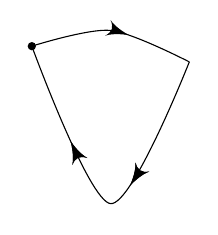
\begin{tikzpicture}[scale=2]
    \draw [->-=0.6] plot [smooth] coordinates {(0, 0) (0.5, 0.1) (1, -0.1)};
    \node [circ] at (0, 0) {};
    \draw [->-=0.4, ->-=0.7] plot [smooth] coordinates {(1, -0.1) (0.5, -1) (0, 0)};
  \end{tikzpicture}
\end{center}

\begin{defi}[Complex integration]
  If $\gamma: [a, b] \to U \subseteq \C$ is $C^1$-smooth and $f: U \to \C$ is continuous, then we define the \emph{integral} of $f$ along $\gamma$ as
  \[
    \int_\gamma f(z) \;\d z = \int_a^b f(\gamma(t)) \gamma'(t) \;\d t.
  \]
  By summing over subdomains, the definition extends to piecewise $C^1$-smooth paths, and in particular contours.
\end{defi}

We have the following properties:
\begin{enumerate}
  \item The definition is insensitive to reparametrization. Let $\phi: [a', b'] \to [a, b]$ be $C^1$ such that $\phi(a') = a, \phi(b') = b$. If $\gamma$ is a $C^1$ path and $\delta= \gamma \circ \phi$, then
    \[
      \int_{\gamma} f(z) \;\d z = \int_{\delta}f(z) \;\d z.
    \]
    This is just the regular change of variables formula, since
    \[
      \int_{a'}^{b'} f(\gamma(\phi(t))) \gamma'(\phi(t)) \phi'(t)\;\d t= \int_a^b f(\gamma(u)) \gamma'(u)\;\d u
    \]
    if $u = \phi(t)$.
  \item If $a < u < b$, then
    \[
      \int_\gamma f(z)\;\d z = \int_{\gamma|_{[a, u]}} f(z)\;\d z + \int_{\gamma|_{[u, b]}}f(z) \;\d z.
    \]
\end{enumerate}
These tells us the integral depends only on the path itself, not how we look at the path or how we cut up the path into pieces.

We also have the following easy properties:
\begin{enumerate}[resume]
  \item If $-\gamma$ is $\gamma$ with reversed orientation, then
    \[
      \int_{-\gamma} f(z)\;\d z = -\int_\gamma f(z)\;\d z.
    \]
  \item If we set for $\gamma: [a, b] \to \C$ the \emph{length}
    \[
      \length(\gamma) = \int_a^b |\gamma'(t)|\;\d t,
    \]
    then
    \[
      \left|\int_\gamma f(z)\;\d z\right| \leq \length (\gamma) \sup_t |f(\gamma(t))|.
    \]
\end{enumerate}

\begin{eg}
  Take $U = \C^*$, and let $f(z) = z^n$ for $n \in \Z$. We pick $\phi: [0, 2\pi] \to U$ that sends $\theta \mapsto e^{i\theta}$. Then
  \[
    \int_\phi f(z)\;\d z =
    \begin{cases}
      2\pi i & n = -1\\
      0& \text{otherwise}
    \end{cases}
  \]
  To show this, we have
  \begin{align*}
    \int_{\phi} f(z)\;\d z &= \int_0^{2\pi} e^{in\theta} ie^{i\theta}\;\d \theta\\
    &= i\int_0^{2\pi} e^{i(n + 1)\theta}\;\d \theta.
  \end{align*}
  If $n = -1$, then the integrand is constantly $1$, and hence gives $2\pi i$. Otherwise, the integrand is a non-trivial exponential which is made of trigonometric functions, and when integrated over $2\pi$ gives zero.
\end{eg}

\begin{eg}
  Take $\gamma$ to be the contour
  \begin{center}
    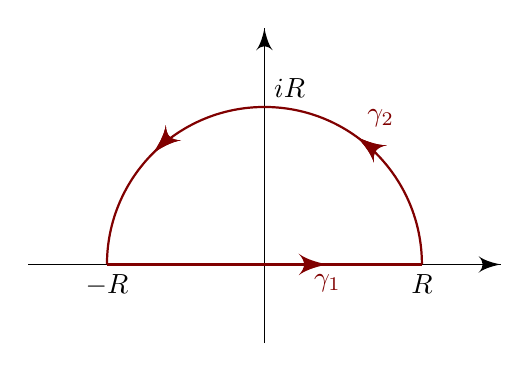
\begin{tikzpicture}
      \draw [->] (-3, 0) -- (3, 0);
      \draw [->] (0, -1) -- (0, 3);
      \draw [thick, mred, ->-=0.7] (-2, 0) -- (2, 0) node [pos=0.7, below] {$\gamma_1$};
      \draw [thick, mred, ->-=0.3, ->-=0.75] (2, 0) arc (0:180:2) node [pos=0.3, anchor = south west] {$\gamma_2$};
      \node [below] at (2, 0) {$R$};
      \node [below] at (-2, 0) {$-R$};
      \node [anchor = south west] at (0, 2) {$iR$};
    \end{tikzpicture}
  \end{center}
  We take the first path to be $\gamma_1: [-R, R] \to \C$ by $\gamma(t) = t$, while $\gamma_2: [0, 1] \to \C$ by $t \mapsto R e^{i\pi t}$.

  Consider the function $f(z) = z^2$. Then the integral is
  \begin{align*}
    \int_\gamma f(z)\;\d z &= \int_{-R}^R t^2 \;\d t + \int_0^1 R^2 e^{2\pi i t} i\pi R e^{i\pi t}\;\d t\\
    &= \frac{2}{3}R^3 + R^3 i\pi \int_0^1 e^{3 \pi i t}\;\d t\\
    &= \frac{2}{3}R^3 + R^3 i\pi \left[\frac{e^{3\pi it}}{3\pi i}\right]_0^1\\
    &= 0
  \end{align*}
\end{eg}
We worked this out explicitly, but this is just an instance of the fundamental theorem of calculus!

\begin{defi}[Antiderivative]
  Let $U \in \C$ and $f: U \to \C$ be continuous. An \emph{antiderivative} of $f$ is a holomorphic function $F: U \to \C$ such that $F'(z) = f(z)$.
\end{defi}

Then the fundamental theorem of calculus tells us:
\begin{thm}[Fundamental theorem of calculus]
  Let $f: U \to \C$ be continuous with antiderivative $F$. If $\gamma: [a, b] \to U$ is piecewise $C^1$-smooth, then
  \[
    \int_\gamma f(z)\;\d z= F(\gamma(b)) - F(\gamma(a)).
  \]
\end{thm}
In particular, the integral depends only on the end points, and not the path itself. Moreover, if $\gamma$ is closed, then the integral vanishes.

\begin{proof}
  We have
  \[
    \int_\gamma f(z)\;\d z = \int_a^b f(\gamma(t)) \gamma'(t) \;\d t = \int_a^b (F \circ \gamma)' (t)\;\d t.
  \]
  Then the result follows from the usual fundamental theorem of calculus, applied to the real and imaginary parts separately.
\end{proof}

\begin{eg}
  This allows us to understand the first example we had. Recall that for $f(z) = z^n$ on $\phi(t) = e^{it}$ (with $0 \leq t \leq 2\pi$), if $n \not= -1$, then
  \[
    f = \frac{\d}{\d t}\left(\frac{z^{n + 1}}{n + 1}\right).
  \]
  So $f$ has a well-defined antiderivative, and the integral vanishes. On the other hand, if $n = -1$, then
  \[
    f(z) = \frac{\d}{\d z} (\log z),
  \]
  where $\log$ can only be defined on a \emph{slit} plane. It is not defined on the whole unit circle. So we cannot apply the fundamental theorem of calculus.

  Reversing the argument around, since $\int_\phi f(z)\;\d z$ does not vanish, this implies there is not a continuous branch of $\log$ on any set $U$ containing the unit circle.
\end{eg}

\begin{prop}
  Let $U \subseteq \C$ be a domain (ie. path-connected non-empty open set), and $f: U \to \C$ be continuous. Moreover, suppose
  \[
    \int_\gamma f(z)\;\d z = 0
  \]
  for any closed piecewise $C^1$-smooth path $\gamma$ in $U$. Then $f$ has an antiderivative.
\end{prop}

This is more-or-less the same proof we gave in IA Vector Calculus that a real function is a gradient if and only if the integral about any closed path vanishes.

\begin{proof}
  Pick our favorite $a_0 \in U$. For $w \in U$, we choose a path $\gamma_w: [0, 1] \to U$ such that $\gamma_w(0) = a_0$ and $\gamma_w(1) = w$. We want to show we can pick $\gamma_w$ such that this is piecewise $C^1$. We already know a \emph{continuous} path $\gamma: [0, 1] \to U$ from $a_0$ to $w$ exists. Since $U$ is open, for all $x$ in the image of $\gamma$, there is some $\varepsilon(x) > 0$ such that $B(x, \varepsilon(x)) \subseteq U$. Since the image of $\gamma$ is compact, it is covered by finitely many such balls. Then it is trivial to pick a piecewise straight path living inside the union of these balls, which is clearly piecewise smooth.

  We thus define
  \[
    F(w) = \int_{\gamma w} f(z)\;\d z.
  \]
  Note that this $F(w)$ is independent of the choice of $\gamma_w$, by our hypothesis on $f$ --- given another choice $\tilde{\gamma}_w$, then $\gamma_w$ concatenated with $-\tilde{\gamma}_w$, written $\gamma_w * (-\tilde{\gamma}_w)$, is a closed piecewise $C^1$ path on $U$. So
  \[
    \int_{\gamma_w * (-\tilde{\gamma}_w)} f(z) \;\d z = 0.
  \]
  The left hand side is
  \[
    \int_{\gamma_W} f(z)\;\d z + \int_{-\tilde{\gamma}_w}f(z)\;\d z = \int_{\gamma_w} f(z)\;\d z - \int_{\tilde{\gamma}_w} f(z) \;\d z.
  \]
  So the two integrals agree.

  Now we need to check that $F$ is complex differentiable. Since $U$ is open, we can pick $\theta > 0$ such that $B(w; \varepsilon) \subseteq U$. Let $\delta_h$ be the radial path in $B(w, \varepsilon)$ from $W$ to $w + h$, with $|h| < \varepsilon$.

  Now note that $\gamma_w * \delta_h$ is a path from $a_0$ to $w + h$. So
  \begin{align*}
    F(w + h) &= \int_{\gamma_w * \delta_h} f(z)\;\d z\\
    &= F(w) + \int_{\delta_h} f(z)\;\d z\\
    &= F(w) + hf(w) + \int_{\delta_h} (f(z) - f(w))\;\d z.
  \end{align*}
  Thus, we know
  \begin{align*}
    \left|\frac{F(w + h) - F(w)}{h} - f(w)\right| &\leq \frac{1}{|h|} \left|\int_{\delta_h} f(z) - f(w)\;\d z\right| \\
    &\leq \frac{1}{|h|} \length(\delta_h) \sup_{\delta_h} |f(z) - f(w)|\\
    &=\sup_{\delta_h} |f(z) - f(w)|.
  \end{align*}
  Since $f$ is continuous, as $h \to 0$, we know $f(z) - f(w) \to 0$. So $F$ is differentiable with derivative $f$.
\end{proof}

In the proof, we constructed the piecewise straight path from $a_0$ to $w$. These paths are nice. In general, we make the following definition:
\begin{defi}[Star-shaped domain]
  A \emph{star-shaped domain} or \emph{star domain} is a domain $U$ such that there is some $p \in U$ such that the line segment $[p, w] \subseteq U$ for all $w \in U$.
  \begin{center}
    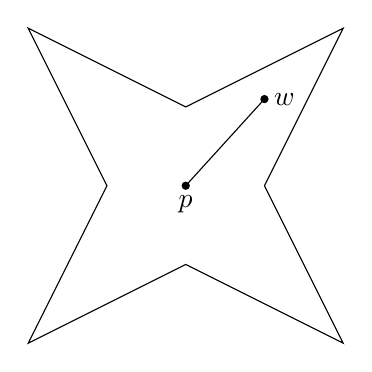
\begin{tikzpicture}
      \draw (1, 0) -- (2, 2) -- (0, 1) -- (-2, 2) -- (-1, 0) -- (-2, -2) -- (0, -1) -- (2, -2) -- (1, 0);
      \node [circ] {};
      \node [below] {$p$};
      \draw (0, 0) -- (1, 1.1) node [circ] {} node [right] {$w$};
    \end{tikzpicture}
  \end{center}
\end{defi}
This is weaker than requiring $U$ to be convex, which says any line segment between \emph{any two points} in $U$, lies in $U$.

Note that we have
\[
  U\text{ is a disc }\Rightarrow U\text{ is convex} \Rightarrow U\text{ is star-shaped} \Rightarrow U\text{ is path-connected},
\]
and none of the implications reverse.

Recall that when constructing the antiderivative, we assumed $\int_\gamma f(z) \;\d z = 0$ for all closed path $\gamma$. We could have required something weaker. All we needed was to intiially pick some $\gamma_w$ for each $w$, and we just need $\int_\gamma f(z)\;\d z = 0$ for all paths of the form $\gamma = \gamma_w * \delta_h * (-\gamma_{w + h})$. If $U$ is a star-shaped domain, then we can pick our pasepoint to be the special point $p$, and then these $\gamma$ are just three straight line segments.

\begin{defi}[Triangle]
  A \emph{triangle} in a domain $U$ is what it ought to be --- the Euclidean convex hull of $3$ points in $U$, lying wholly in $U$. We write its boundary as $\partial T$, which we view as an oriented piecewise $C^1$ path, ie. a contour.
\end{defi}
\begin{center}
  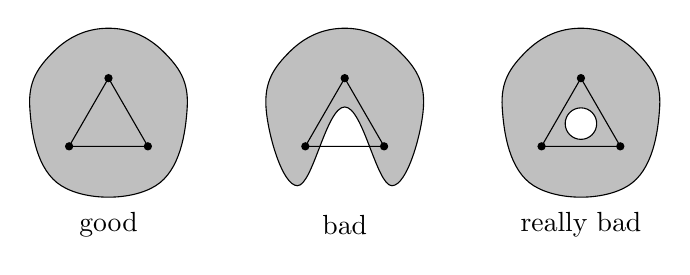
\begin{tikzpicture}
    \begin{scope}[shift={(-3, 0)}]
      \draw [fill=gray!50!white] plot [smooth cycle, tension=0.7] coordinates {(0, 1) (-0.7, 0.7) (-1, 0) (-0.6, -1) (0.6, -1) (1, 0) (0.7, 0.7)};
      \draw (-0.5, -0.5) node [circ] {} -- (0.5, -0.5) node [circ] {} -- (0, 0.366) node [circ] {} -- cycle;

      \node at (0, -1.5) {good};
    \end{scope}

    \begin{scope}
      \draw [fill=gray!50!white] plot [smooth cycle, tension=0.7] coordinates {(0, 1) (-0.7, 0.7) (-1, 0) (-0.6, -1) (0, 0) (0.6, -1) (1, 0) (0.7, 0.7)};
      \draw (-0.5, -0.5) node [circ] {} -- (0.5, -0.5) node [circ] {} -- (0, 0.366) node [circ] {} -- cycle;

      \node at (0, -1.5) {bad};
    \end{scope}

    \begin{scope}[shift={(3, 0)}]
      \draw [fill=gray!50!white] plot [smooth cycle, tension=0.7] coordinates {(0, 1) (-0.7, 0.7) (-1, 0) (-0.6, -1) (0.6, -1) (1, 0) (0.7, 0.7)};
      \draw (-0.5, -0.5) node [circ] {} -- (0.5, -0.5) node [circ] {} -- (0, 0.366) node [circ] {} -- cycle;
      \draw [fill=white] (0, -0.2113) circle [radius=0.2];

      \node at (0, -1.5) {really bad};
    \end{scope}
  \end{tikzpicture}
\end{center}
Our earlier result on constructing antiderivative shows:
\begin{prop}
  If $U$ is a star domain, and $f: U \to \C$ is continuous, and if
  \[
    \int_{\partial T} f(z)\;\d z = 0
  \]
  for all triangles $T \subseteq U$, then $f$ has an antiderivative on $U$.
\end{prop}

\begin{proof}
  As before, taking $\gamma_w = [a_0, w] \subseteq U$ if $U$ is star-shaped about $a_0$.
\end{proof}

This is in some sense a weaker proposition --- while our hypothesis only requires the integral to vanish over triangles, and not arbitrary closed loops, we are restricted to star domains only.

It turns out triangles are in general nice:
\begin{thm}[Cauchy's theorem for a triangle]
  Let $U$ be a domain, and let $f: U \to \C$ be holomorphic. If $T \subseteq U$ is a triangle, then $\int_{\partial T} f(z)\;\d z = 0$.
\end{thm}
So for holomorphic functions, the hypothesis of the previous theorem automatiaclly holds.

We immediately get the following corollary, which is what we will end up using most of the time.
\begin{cor}[Convex Cauchy]
  If $U$ is a convex or star-shaped domain, and $f: U \to \C$ is holomorphic, then for \emph{any} closed piecewise $C^1$ paths $\gamma \in U$, we must have
  \[
    \int_\gamma f(z)\;\d z = 0.
  \]
\end{cor}

\begin{proof}(of corollary)
  If $f$ is holomorphic, then Cauchy's theorem says the integral over any triangle vanishes. If $U$ is star shaped, our proposition says $f$ has an antiderivative. Then the fundamental theorem of calculus tells us the integral around any closed path vanishes.
\end{proof}

Hence, all we need to do is to prove that fact about triangles.
\begin{proof}(of Cauchy's theorem for a triangle)
  Fix a triangle $T$. Let
  \[
    \eta = \left|\int_{\partial T} f(z)\;\d z\right|, \ell = \length (\partial T).
  \]
  The idea is to show for any $\varepsilon > 0$ that $\eta < \varepsilon$, and hence we must have $\varepsilon = 0$. To do so, we subdivide our triangles.

  Before we start, it helps to motivate the idea of subdividing a bit. By subdividing the triangle further and further, we are focusing on a smaller and smaller region of the complex plane. This allows us to study how the integral behaves locally. This is helpful since we are given that $f$ is holomorphic, and holomorphicity is a local property.

  We start with $T = T^0:$
  \begin{center}
    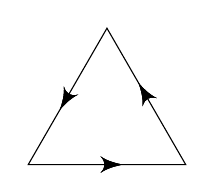
\begin{tikzpicture}
      \draw [->-=0.2, ->-=0.533, ->-=0.866] (0, 0) -- (2, 0) -- (1, 1.732) -- cycle;
    \end{tikzpicture}
  \end{center}
  We then add more lines to get $T_a^0, T_b^0, T_c^0, T_d^0$ (it doesn't really matter which is which).
  \begin{center}
    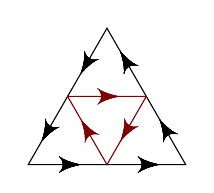
\begin{tikzpicture}
      \draw [->-=0.112, ->-=0.279, ->-=0.445, ->-=0.612, ->-=0.779, ->-=0.945] (0, 0) -- (2, 0) -- (1, 1.732) -- cycle;
      \draw [mred, ->-=0.22, ->-=0.553, ->-=0.886] (1, 0) -- (0.5, 0.866) -- (1.5, 0.866) -- cycle;
    \end{tikzpicture}
  \end{center}
  Then we have
  \[
    \int_{\partial T^0} f(z)\;\d z = \sum_{a, b, c, d} \int_{\partial T^0_{\Cdot}} f(z)\;\d z,
  \]
  if we orient the middle triangle by the anticlockwise orientation, as then each internal edge occurs twice, with opposite orientation.

  For this to be possible, if $\eta = \left|\int_{\partial T^0} f(z)\;\d z\right|$, then there must be some subscript in $\{a, b, c, d\}$ such that
  \[
    \left|\int_{\partial T^0_{\Cdot}} f(z)\;\d z\right| \geq \frac{\eta}{4}.
  \]
  We call this $T_{\Cdot}^0 = T^1$. Then the length of $\partial T^1$ has length
  \[
    \length(\partial T^0_{\Cdot}) = \frac{\ell}{2}.
  \]
  Iterating this, we obtain triangles
  \[
    T^0 \supseteq T^1 \supseteq T^2 \supseteq \cdots
  \]
  such that
  \[
    \left|\int_{\partial T^i} f(z)\;\d z\right| \geq \frac{\eta}{4^i},\quad \length (\partial T^i) = \frac{\ell}{2^i}.
  \]
  Now we are given a nested sequence of closed sets. By IB Metric and Topological Spaces (or IB Analysis II), there is some $z_0 \in \bigcap_{i \geq 0} T^i$.

  Now fix an $\varepsilon > 0$. Since $f$ is holomorphic at $z_0$, we can find a $\delta > 0$ such that
  \[
    |f(w) - f(z_0) - (w - z_0) f'(z_0)| \leq \varepsilon|w - z_0|
  \]
  whenever $|w - z_0| < \delta$. Since the diameters of the triangles are shrinking each time, we can pick an $n$ such that $T^n \subseteq B(z_0, \varepsilon)$. We're almost there. We just need to do one last thing that is slightly sneaky. Note that
  \[
    \int_{\partial T^n} 1 \;\d z = 0 = \int_{\partial T^n} z \;\d z,
  \]
  since these functions certainly do have antiderivatives on $T^n$. Therefore, noting that $f(z_0)$ and $f'(z_0)$ are just constants, we have
  \begin{align*}
    \left|\int_{\partial T^n}f(z)\;\d z\right| &= \left|\int_{\partial T^n} (f(z) - f(z_0) - (z - z_0) f'(z_0))\;\d z\right|\\
    &\leq \int_{\partial T^n} |f(z) - f(z_0) - (z - z_0) f'(z_0)|\;\d z\\
    &\leq \length(\partial T^n) \varepsilon \sup_{z \in \partial T^n}|z - z_0|\\
    &\leq \varepsilon \length(\partial T^n)^2,
  \end{align*}
  since $z_0 \in T^n$, and the distance between any two points in the triangle cannot be greater than the perimeter of the triangle. Substituting our fomulas for these in, we have
  \[
    \frac{\eta}{4^n}\leq \frac{1}{4^n} \ell^2 \varepsilon.
  \]
  So
  \[
    \eta \leq \ell^2 \varepsilon.
  \]
  Since $\ell$ is fixed and $\varepsilon$ was arbitrary, it follows that we must have $\eta = 0$.
\end{proof}
Is this the best we can do? Can we formulate this for an arbitrary domain, and not just star-shaped ones? It is obviously not true if the domain is not simply connected, eg. for $f(z) = \frac{1}{z}$ defined on $\C \setminus \{0\}$. However, it turns out Cauchy's theorem holds as long as the domain is simply connected, but we probably won't get to prove that. However, this is not surprising given the Riemann mapping theorem, since any simply connected domain is conformally eequivalent to the unit disk.

\end{document}
